\section{Systemarkitektur}
I dette kapitel vil systemarkitekturen for winePrep blive beskrevet. Arkitekturen vil blive delt op i hardware og software og tager udgangspunkt 
i de UML-/SysML-diagrammer, der er lavet over systemet. 

\subsection{Hardware}
I BDD'et for winePrep ses hvilke hardwareblokke systemet består af. I dette afsnit vil disse hardwareblokke og deres funktion i systemet blive beskrevet.
Systemet indeholder tre CPU'er, DevKit8000, PSoC-Master og PSoC-Slave. Herudover er der en strømforsyning, åbningsmekanisme og positionering. \\

\begin{figure}[H]
	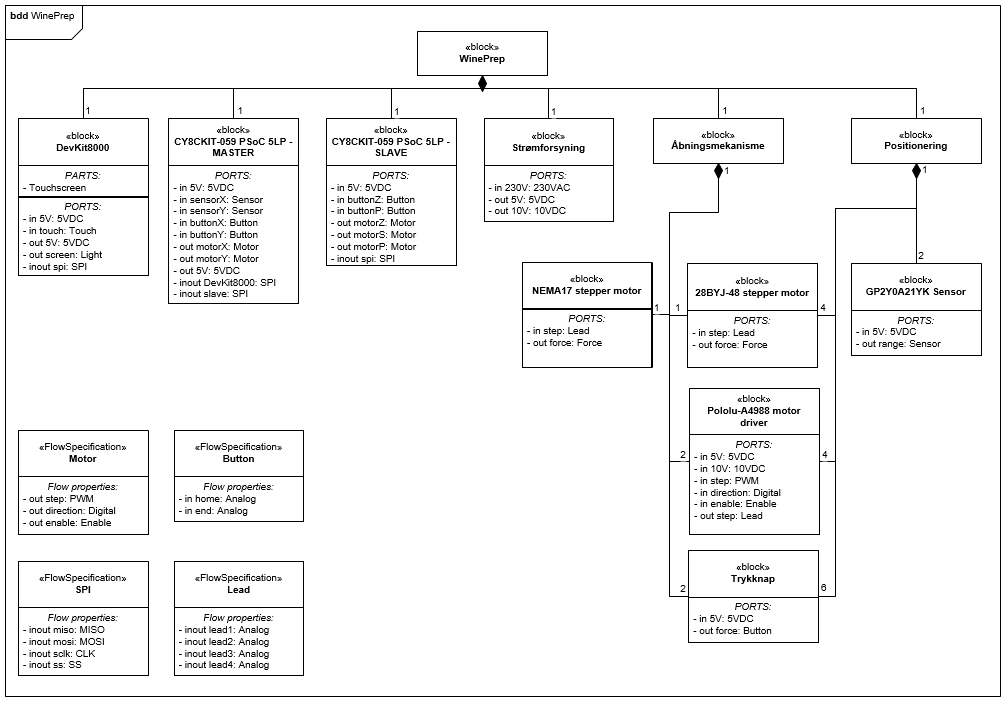
\includegraphics[scale=0.33]{tex/Arkitektur/Fotos/HW/BDD_winePrep}
	\caption{BDD for WinePrep}
\end{figure}

\subsubsection{Åbningsmekanisme:}
Til selve åbningen af en vinflaske er der konstrueret en åbningsmekanisme. Den indeholder to motorer, en til iskruning, og en til optrækning.
For at kunne holde styr på skruens position, er der implementeret to trykknapper, der indikerer start og slut position. Motorene bliver styret via 
pololu motor drivere(INDSÆT REFERENCE TIL POLOLU). \\   

\subsubsection{Positionering:}
For at detektere vinflaskens position og positionere åbningsmekanismen korrekt, anvendes en positioneringsmekanisme. Herpå er monteret to motorer som finder
vinflaskens x- og y-koordinator vha. sensorer. Z-koordinatet bliver reguleret af yderligere to motorer, som hæver og sænker åbningsmekanismen. 
Der er implementeret to trykknapper, en som indikerer at åbningsmekanismen er tilstrækkelig tæt på vinflaskens åbning, den anden indikerer startpositionen. 
Yderligere fire trykknapper indikerer at x-/y-motorerne har nået deres yderposition. Alle motorene bliver ligeledes styret via pololu motor drivere. \\

\subsubsection{DevKit8000:}
Dette er et prototypekit, hvorpå Linux distribution ångström er installeret. Det er via DevKit8000's touchskærm at interaktion med brugeren foregår. 
Denne enhed har dermed til opgave at tage imod input fra brugeren og sende disse videre i systemet, samt at give brugeren status beskeder. Den er forbundet til PSoC-Master via en SPI forbindelse. \\

\subsubsection{PSoC-Master:}
PSoC er en programmerbar CPU-enhed med GPIO pins, som har ansvaret for styring/aflæsning af hardware enheder. PSoC-Master er forbundet til positionering, 
hvor den styrer x-/y-motorer via pololu motor drivere, og aflæser x-/y-sensorer samt x-/y-trykknapper. Den er forbundet med PSoC-Slave via SPI. \\

\subsubsection{PSoC-Slave:}
Denne enhed styrer via pololu motor drivere de to z motorer på positionering, samt motorene på åbningsmekanismen. Den aflæser også z trykknapper på 
positionering og trykknapper på åbningsmekanismen. \\

\subsubsection{Strømforsyning:}
Denne enhed leverer strøm til de enkelte hardware blokke. De tre CPU'er skal hver have 5 volt, det samme skal sensorer og trykknapper. Pololu motor driverne 
skal have både 5 og 10 volt. \\

\subsection{Software}
I dette afsnit vil arkitekturen for systemets software blive beskrevet.
Systemet indeholder som tidligere nævnt tre CPU'er, hvorpå der er allokeret software til interaktion med brugeren samt styring/aflæsning af diverse 
motorer, sensorer og trykknapper. På figur \ref{AlDi} ses denne allokering af software på de respektive hardware blokke. \\

\begin{figure}[H]
	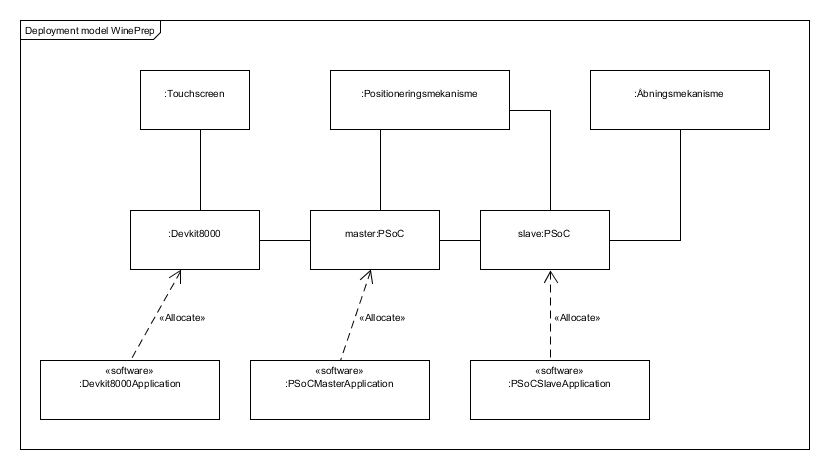
\includegraphics[scale=0.4]{tex/Arkitektur/Fotos/SW/Allokeringsdiagram}
	\caption{Software allokeringsdiagram for winePrep}
	\label{AlDi}
\end{figure}  

\subsubsection{DevKit8000 (Linux platform)}
DevKit8000 har ansvaret for interaktion med brugeren via touchskærm. Derfor har systemet brug for en grafisk brugergrænseflade (GUI), hvorpå der er
implementeret virtuelle knapper, som gør det muligt at oversætte de fysiske tryk til kommandoer, der kan sendes videre i systemet. Der skal også kunne vises
status beskeder til brugeren, så denne er klar over systemets tilstand. Dette implementeres vha. viduer med tekstbeskeder. For at kunne sende brugerinputs 
videre i systemet skal DevKit8000 forbindes til PSoC-Master via SPI. Da der køres med Linux på DevKit8000 kræves det derfor at en SPI device driver bliver
indsat i kernen. DevKit8000 har altså to boundary klasser, som viser grænsefladerne for DevKit8000. I klassediagramet ses også en protokolklasse for SPI, denne 
indeholder blot information til dekodning af de bits som bliver sendt over SPI. \\

\begin{figure}[H]
	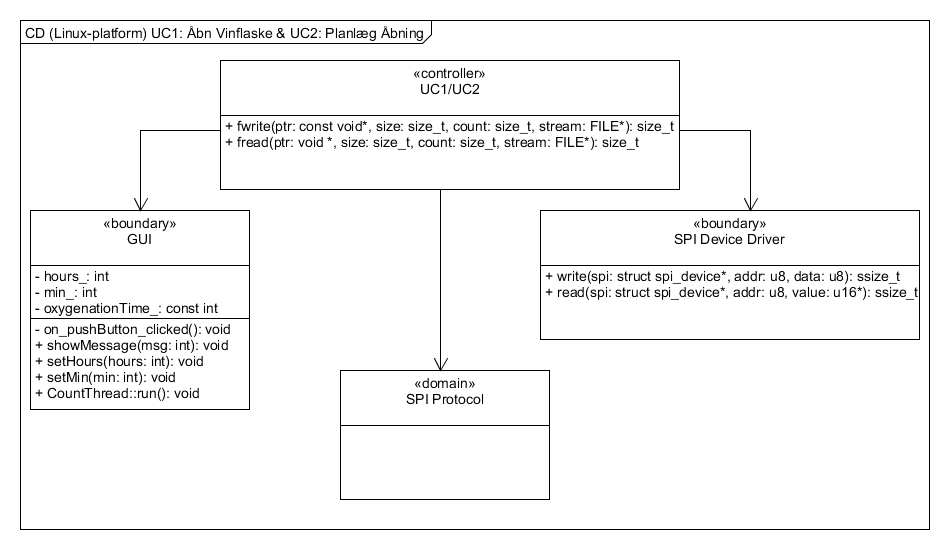
\includegraphics[scale=0.4]{tex/Arkitektur/Fotos/SW/Klassediagram_Linuxplatform}
	\caption{Klassediagram DevKit8000}
\end{figure}

Med udgangpunkt i usecasen "Åbn Vinflaske", vil interaktionen mellem DevKit8000 og boundary-klasserne blive beskrevet. 
GUI repræsenterer her grænsefladen til brugeren, og når denne trykker på en virtuel knap, kaldes write metoden fra controllerklassen, som skriver den korrekte 
kommando ud til SPI device driveren. Læsning fra SPI device driveren indledes også fra GUI, og når controller-klassen har læst data, sendes status beskeder 
tilbage til GUI, og dermed informeres brugeren. \\

\begin{figure}[H]
	\includegraphics[scale=0.4]{tex/Arkitektur/Fotos/SW/Sekvensdiagram_åbnvinflaske_Linuxplatform}
	\caption{Sekvensdiagram for usecasen "Åbn Vinflaske" på DevKit8000}
\end{figure}

\subsubsection{PSoC-Master og PSoC-Slave}
PSoC-Master og PSoC-Slave vil blive beskrevet under samme afsnit da de deler klasse- og sekvensdiagrammer. 
Grunden til de ikke er opdelt er for overskueligehedens skyld. Da PSoC-enhederne deler ansvaret for styring af positionering, giver det mening at de er 
indkluderet i samme sekvensdiagram. Det vil sige at der er to controllerklasser i klasse- og sekvensdiagrammerne. \\

PSoC-Master har to SPI boundary klasser, en til kommunikation med DevKit8000, og en til PSoC-Slave. Herudover er der boundary klasser til x/y motorer og 
sensorer på positionering. 
PSoC-Slave har SPI boundary klasse til kommunikation med PSoC-Master og til z-motorer på positionering, og motorer på åbningsmekanismen. Begge PSoC-enheder har
en SPI-protokol til dekodning af SPI-kommandoer. \\

\begin{figure}[H]
	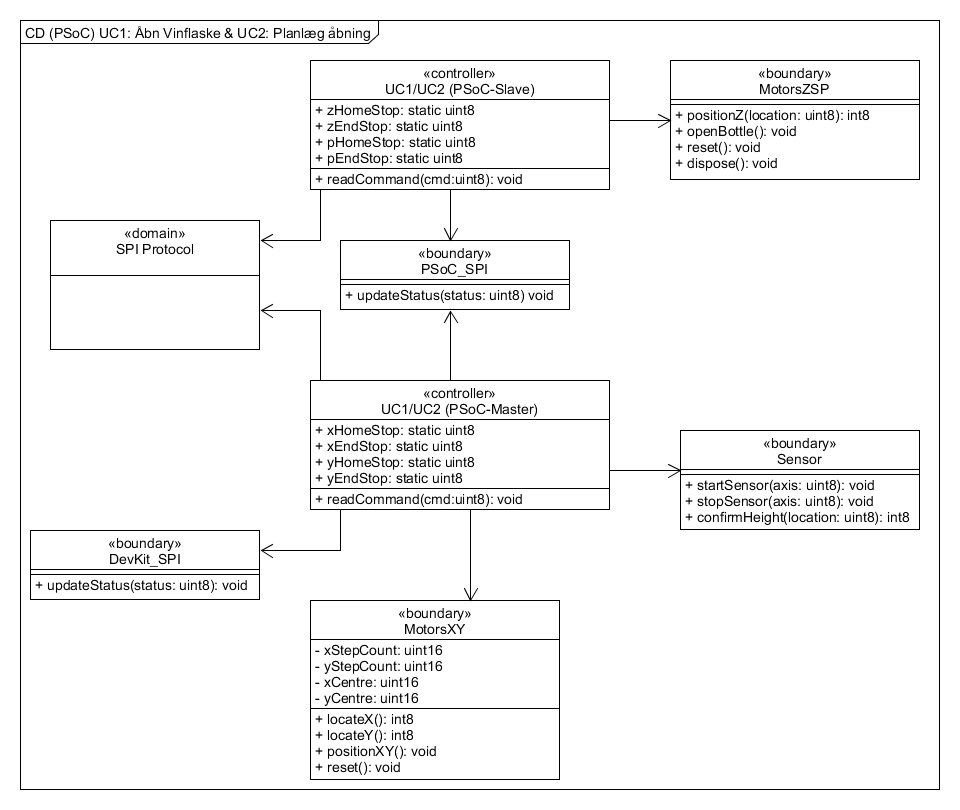
\includegraphics[scale=0.4]{tex/Arkitektur/Fotos/SW/Klassediagram_PSoC}
	\caption{Klassediagram PSoC-Master/-Slave}
\end{figure}

Usecasene "Åbn Vinflaske" og "Planlæg Åbning" er samlet under det samme sekvensdiagram (se figur \ref{SD_PSoC}), da der fra PSoC-enhedernes synspunkt sker det samme, nemlig 
åbning af en vinflaske. Timing af åbningen foregår på DevKit8000, og har ingen relevans for PSoC-enhederne. Der er ikke medtaget alternative scenarier i 
sekvensdiagrammet, da disse er trivielle, og blot skaber unødvendig uoverskuelighed. \\

Selve åbningen initieres fra SPI-forbindelsen til DevKit8000. Herefter
sætter PSoC-Master x-/y-motorer til vha. sensorerne at finde flaskens x-/y-placering. Når disse er fundet, gives der besked til PSoC-Slave om at aktivere z-motorerne
og finde den rette afstand til flaskens top. Når denne er fundet påbegyndes åbningen af vinflasken, og derefter dispensering af proppen. Sekvensdiagrammet
afsluttes med en retur besked tilbage til DevKit8000 via SPI om succesfuld åbning.

\begin{figure}[H]
	\centerline{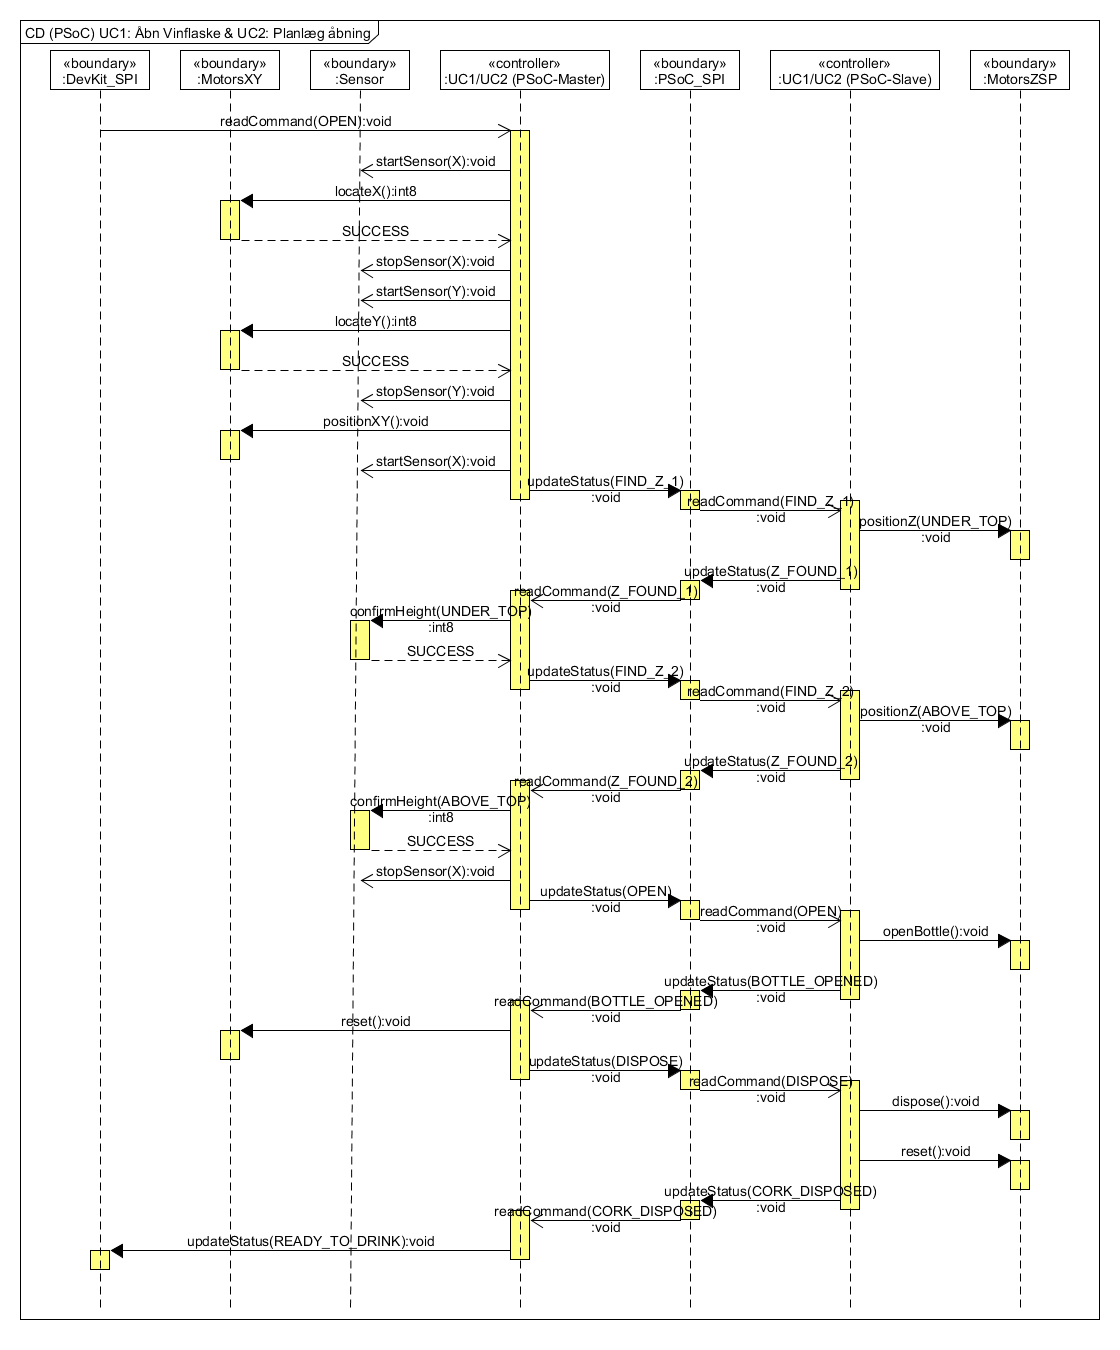
\includegraphics[scale=0.4]{tex/Arkitektur/Fotos/SW/Sekvendiagram_PSoC}}
	\caption{Sekvensdiagram PSoC-Master/-Slave}
	\label{SD_PSoC}
\end{figure}